\documentclass[aspectratio=169%可调屏宽比16:9(169),4:3(43)
,serif,mathserif]{beamer}
\mode<presentation>{
%\usetheme{default}
%\usetheme{AnnArbor}
%\usetheme{Antibes}
%\usetheme{Bergen}
%\usetheme{Berkeley}
%\usetheme{Berlin}
%\usetheme{Boadilla}
%\usetheme{CambridgeUS}
%\usetheme{Copenhagen}
%\usetheme{Darmstadt}
%\usetheme{Dresden}
%\usetheme{Frankfurt}
%\usetheme{Goettingen}
%\usetheme{Hannover}
%\usetheme{Ilmenau}
%\usetheme{JuanLesPins}
%\usetheme{Luebeck}
\usetheme{Madrid}
%\usetheme{Malmoe}
%\usetheme{Marburg}
%\usetheme{Montpellier}
%\usetheme{PaloAlto}
%\usetheme{Pittsburgh}
%\usetheme{Rochester}
%\usetheme{Singapore}
%\usetheme{Szeged}
%\usetheme{Warsaw}
% As well as themes, the Beamer class has a number of color themes
% for any slide theme. Uncomment each of these in turn to see how it
% changes the colors of your current slide theme.
%\usecolortheme{albatross}
%\usecolortheme{beaver}
%\usecolortheme{beetle}
%\usecolortheme{crane}
%\usecolortheme{dolphin}
%\usecolortheme{dove}
%\usecolortheme{fly}
%\usecolortheme{lily}
%\usecolortheme{orchid}
%\usecolortheme{rose}
%\usecolortheme{seagull}
%\usecolortheme{seahorse}
%\usecolortheme{whale}
%\usecolortheme{wolverine}
%\setbeamertemplate{footline} % To remove the footer line in all slides uncomment this line
%\setbeamertemplate{footline}[page number] % To replace the footer line in all slides with a simple slide count uncomment this line
%\setbeamertemplate{navigation symbols}{} % To remove the navigation symbols from the bottom of all slides uncomment this line
}
\usepackage{adjustbox}
\usepackage{indentfirst} 
\usepackage{amsmath, amsfonts, epsfig, xspace}
\usepackage{algorithm,algorithmic}
\usepackage{beamerthemesplit}
\usepackage{booktabs}
\usepackage{bm}
\usepackage{braket}
\usepackage{calligra}
\usepackage[T1]{fontenc}
\usepackage{fontspec}
\usepackage{ctex}
\usepackage{latexsym}
\usepackage{multicol}
\usepackage{multimedia}
\usepackage{calligra} \DeclareMathAlphabet{\mathcalligra}{T1}{calligra}{m}{n} \DeclareFontShape{T1}{calligra}{m}{n}{<->s*[2.2]callig15}{}
\usepackage{pstricks,pst-node}
\usepackage{ragged2e}
\usepackage{setspace}
\usepackage[normal,tight,center]{subfigure}
\setlength{\subfigcapskip}{-.5em}
\setlength{\parindent}{2em}
\begin{document}
\title{Integrating Simplex with DPLL(T)} % The short title appears at the bottom of every slide, the full title is only on the title page
\author[迟智名]{Reporter:~Chi~Zhiming} % Your name
\institute[ISCAS] % Your institution as it will appear on the bottom of every slide, may be shorthand to save space
{	
	%Lanzhou University \\ % Your institution for the title page
	%\medskip
	%\textit{chizhm16@lzu.edu.cn} % Your email address
}
	\CTEXoptions[today=old]
	\date{\today} % Date, can be changed to a custom date
\begin{frame}[plain]\vspace{1.5em}
\titlepage\vspace{-0.5cm}
%\centerline{\includegraphics[height=0.30\textheight]{logo.png}}
%\hfill 指导教师:xxx
\end{frame}
\begin{frame}{目录}
\tableofcontents
\end{frame}
\AtBeginSection[]
{
\begin{frame}{\tiny}
\frametitle{目录}
\tableofcontents[currentsection]
\end{frame}
}
%----------------------------------------------------------------------------------------
%	PRESENTATION SLIDES
%----------------------------------------------------------------------------------------

%------------------------------------------------
\section{Introduction} % Sections can be created in order to organize your presentation into discrete blocks, all sections and subsections are automatically printed in the table of contents as an overview of the talk
%------------------------------------------------
\begin{frame}
	\frametitle{Contribution}
	\begin{itemize}
		\item We have presented a new Simplex-based solver designed for efficiently solving SMT problems in solving linear arithmetic.
		\item The main features of the new approach include the possibility to presimplify the input problem by eliminating variables, a reduction in the number of slack variables, and fast backtracking.
		\item Another result of the paper is a simple approach for solving strict inequalities that does not require modification of the basic Simplex algorithm.
	\end{itemize}

\end{frame}

\section{Background}
\begin{frame}
	\frametitle{DPLL(T) approach}
	If $\phi$ is a formula built by boolean combination of atoms of quantifier-free theory $T$, then the
	satisfiability of $\phi$ can be decided by combining a boolean satisfiability solver and a $T-solver$.
	\begin{itemize}
		\item First $\Phi$ is transformed into a propositional formula $\Phi_{0}$ by replacing its atoms $\phi_{1}, \ldots, \phi_{t}$ with fresh propositions $p_{1}, \ldots, p_{t}$
		\item A boolean valuation for $\Phi_{0}$ is a mapping $b$ from $\Phi_{0}$ 's propositions to $\{0,1\}$. Any such $b$ defines a set of atoms $\Gamma_{b}=\left\{\gamma_{1}, \ldots, \gamma_{t}\right\}$ where $\gamma_{i}$ is $\phi_{i}$ if $b\left(p_{i}\right)=1$ and $\gamma_{i}$ is $\neg \phi_{i}$ if $b\left(p_{i}\right)=0$. 
		\item Then $\Phi$ is satisfiable if there is a $b$ that satisfies $\Phi_{0}$ (in propositional logic) and for which $\Gamma_{b}$ is consistent (in theory $T$ ).
	\end{itemize}
\end{frame}

\begin{frame}
	\frametitle{Solvers for DPLL(T):~Terminology}
	\begin{itemize}
		\item State:, a $T-solver$ maintains a \textbf{state} that is an internal representation of the
		atoms asserted so far. \\
		      This solver must provide operations for updating the state by asserting new
		atoms, checking whether the state is consistent, and for backtracking.
		\item Theory propagation: identify atoms that are implied by the current state.
		\item Explanation:
			\begin{itemize}
				\item In an inconsistent state $S$, an explanation is any inconsistent subset of the atoms asserted in $S$.
				\item Similarly, an explanation for an implied atom $\gamma$ is a subset $\Gamma$ of the asserted atoms such that $\Gamma \models \gamma$. 
			\end{itemize}
			To interact with the DPLL search, the solver must produce explanations for conflicts and propagated atoms
		\item Minimal: In both above cases, the explanation is \textbf{minimal} if no proper subset of $\Gamma$ is itself an explanation.
	
	\end{itemize}	

\end{frame}

\begin{frame}
	\frametitle{General Settings}		

		Initial:
			\begin{itemize}
				\item fixed formula $\phi$.
				\item The set of atoms asserted so far is denoted by $\alpha$.
				\item Stack of checkpoints: mark consistent states to which the solver can backtrack.
			\end{itemize}

\end{frame}


\begin{frame}
	\frametitle{General Settings}	
	API:
	\begin{itemize}
		\item \emph{Assert($\gamma$)}:~asserts atom $\gamma$ in the current state. It returns either ok or unsat $\langle\Gamma\rangle$ where $\Gamma$ is a subset of $\alpha$. In the first case, $\gamma$ is inserted into $\alpha$. In the latter case, $\alpha \cup\{\gamma\}$ is inconsistent and $\Gamma$ is the explanation.
		\item \emph{Check()}:~checks whether $\alpha$ is consistent. If so, it returns ok, otherwise it returns unsat $\langle\Gamma\rangle$. As previously $\Gamma \subseteq \alpha$ is an explanation for the inconsistency. A new checkpoint is created when ok is returned.
		\item \emph{Backtrack()}:~backtracks to the consistent state represented by the checkpoint on the top of the stack.
		\item \emph{Propagate()}:~performs theory propagation. It returns a set $\left\{\left\langle\Gamma_{1}, \gamma_{1}\right\rangle, \ldots,\left\langle\Gamma_{t}, \gamma_{t}\right\rangle\right\}$ where $\Gamma_{i} \subseteq$ $\alpha$ and $\gamma_{i} \in \mathcal{A} \backslash \alpha$. Every $\gamma_{i}$ is implied by $\Gamma_{i}$
	\end{itemize}
\end{frame}

\begin{frame}
	\frametitle{General Settings}	
	\begin{itemize}
		\item \emph{Assert} must be sound but is not required to be complete: $Assert(\gamma)$ may return ok even if $\alpha \cup \{\gamma\}$ is inconsistent.
		\item \emph{Propagate} must be sound but does not have to be exhaustive.A solver without theory propagation can return $Propagate()=\emptyset$ for any $S$
		\item \emph{Check} is required to be sound and complete
		\item Several calls to \emph{Assert} followed by a single call to \emph{Check}.
		\item The state $S'$ after executing Backtrack must be logically equivalent
		to the state $S$ when the checkpoint was created, but $S'$ may be different from $S$.
	\end{itemize}
\end{frame}

\section{A Linear-Arithmetic Solver for DPLL(T)}
\subsection{Preprocessing}
\begin{frame}
	\frametitle{Preprocessing}
	Rewriting: $\phi$ into an equisatisfiable formula of the form $\phi_A \wedge \phi'$
	\begin{itemize}
		\item $\phi_A$ is a conjunction of linear equalities
		\item $\phi'$ are \textbf{elementary atoms} of the form $y \bowtie b$, where $y$ is a variable and $b$ is a rational constant. 
	\end{itemize}

	$$
		x \geq 0 \wedge(x+y \leq 2 \vee x+2 y-z \geq 6) \wedge(x+y=2 \vee x+2 y-z>4) 
	$$

	$\iff$

	$$
	\begin{gathered}
		\left(s_{1}=x+y \wedge s_{2}=x+2 y-z\right) \wedge \\
		\left(x \geq 0 \wedge\left(s_{1} \leq 2 \vee s_{2} \geq 6\right) \wedge\left(s_{1}=2 \vee s_{2}>4\right)\right)
	\end{gathered}
	$$

\end{frame}

\begin{frame}
	\frametitle{Preprocessing}
	\begin{itemize}
		\item Then $\phi_A$ can be written in matrix form as $Ax = 0$.
		\item checking the satisfiability of $\phi$ in linear arithmetic $\iff$ checking the satisfiability of $\phi'$ in \textbf{linear arithmetic modulo} $Ax = 0$.
		\item Solver: deciding the consistency of a set of elementary atoms $\Gamma$ modulo the constraints $Ax = 0$
		\item If $\Gamma$ contains only equalities and (non-strict) inequalities,this problem can reduce to search $x \in R$ for:
			\begin{equation}
				A x=0 \text { and } l_{j} \leq x_{j} \leq u_{j} \text { for } j=1, \ldots, n
			\end{equation}
	\end{itemize}
\end{frame}

\begin{frame}
	\frametitle{Preprocessing}
	\begin{itemize}
		\item Reduce the matrix size: Simplify the costraints $Ax = 0$ by removing any variable $x_i$ that does not occur in any elementary atom of $\phi'$ by Gaussian elimination.
		\item the presence of both lower and upper bounds is beneficial
	\end{itemize}
\end{frame}

\begin{frame}
	\frametitle{Basic Solver}
	Initial:
	\begin{itemize}
		\item Tableau: From $Ax = 0$,
			$$
			x_{i}=\sum_{x_{j} \in \mathcal{N}} a_{i j} x_{j} \quad x_{i} \in \mathcal{B},
			$$
		\item $\beta$: assigns a rational value $\beta(x_i)$ to every variable $x_i$; $\beta_0(x_j) = 0$
		\item Bound: $l_j = -\infty, u_j = \infty$ for all $j$
		\item Invariants: $\forall x_{j} \in \mathcal{N}, l_{j} \leq \beta\left(x_{j}\right) \leq u_{j}$
	\end{itemize}
\end{frame}

\begin{frame}
	\frametitle{Basic Solver}
	Two auxiliary procedures that modify $\beta$:
	\begin{figure}[htbp]
		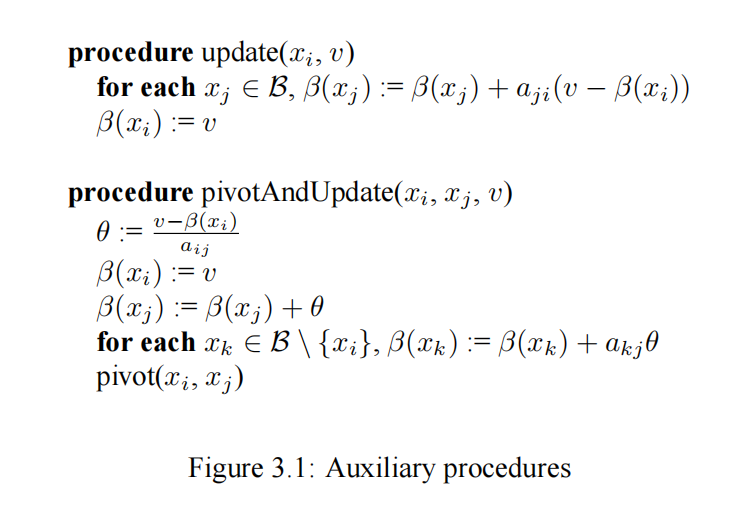
\includegraphics[width=.6\linewidth]{1.png}
	\end{figure}
\end{frame}

\subsection{Main algorithm}
\begin{frame}
	\frametitle{Assertion Procedures}
	We use these two procedures to update the bounds $l_i$ and $u_i$.
	\begin{figure}[htbp]
		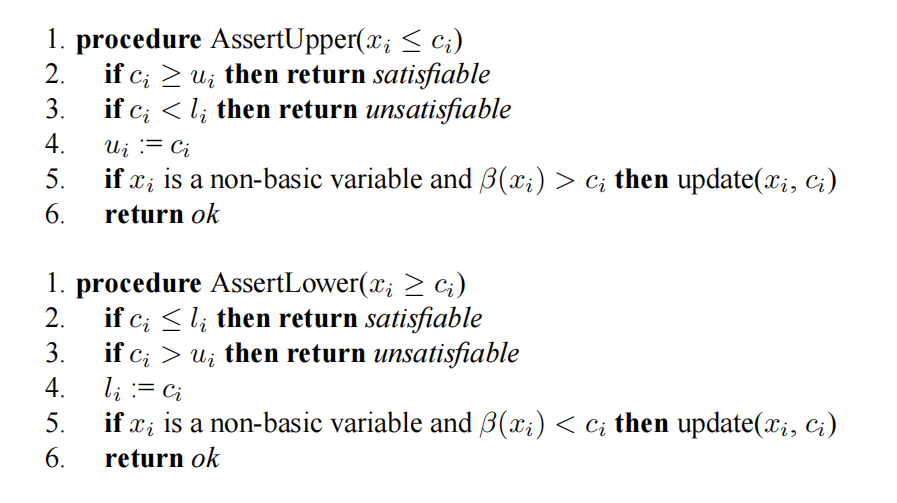
\includegraphics[width=.6\linewidth]{2.png}
	\end{figure}
	An equality $x_i = c_i$ is asserted by calling both \emph{AssertLower} and \emph{AssertUpper}.
\end{frame}

\begin{frame}
	\frametitle{Check}
	Modify the $\beta(x_i)$ for basic variable $x_i$ such that $l_{i} \leq \beta\left(x_{i}\right) \leq u_{i}$
	\begin{figure}[htbp]
		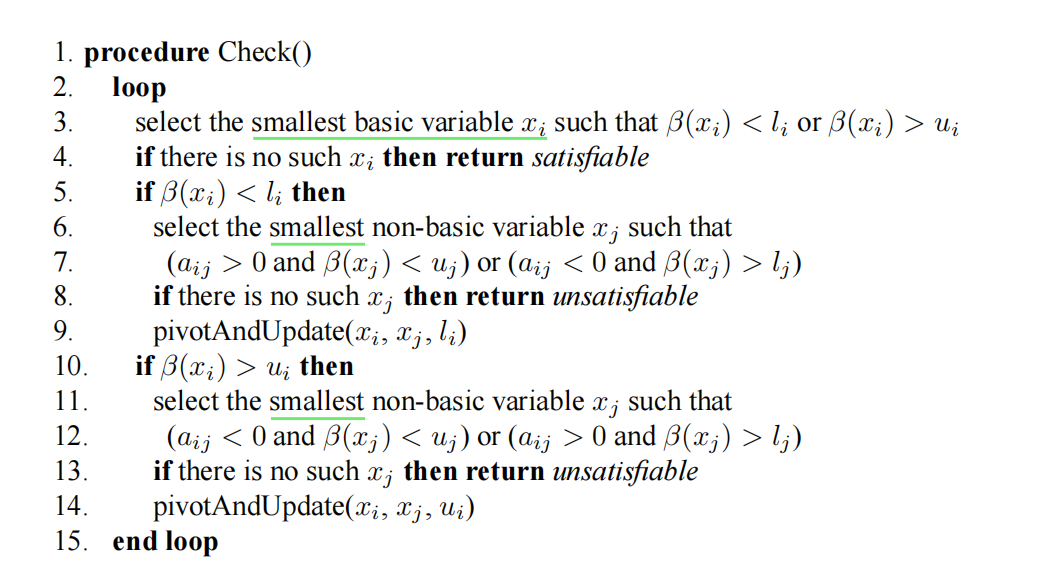
\includegraphics[width=.7\linewidth]{3.png}
	\end{figure}

\end{frame}

\begin{frame}
	\frametitle{Generating Explanations}
	An inconsistency may be detected by \emph{Check} at line 8 or 13. Assume at line 8:
	\begin{itemize}
		\item Basic variable $x_i$ such that $\beta\left(x_{i}\right)<l_{i} \implies a_{i j}>0 \Rightarrow \beta\left(x_{j}\right) = u_{j} \text { and } a_{i j}<0 \Rightarrow \beta\left(x_{j}\right) = l_{j}$ for all non-basic variable $x_j$
		\item It follows that: Let $ \mathcal{N}^{+}=\left\{x_{j} \in \mathcal{N} \mid a_{i j}>0\right\},\text { Let } \mathcal{N}^{-}=\left\{x_{j} \in \mathcal{N} \mid a_{i j}<0\right\}$
			$$
			\beta\left(x_{i}\right)=\sum_{x_{j} \in \mathcal{N}} a_{i j} \beta\left(x_{j}\right)=\sum_{x_{j} \in \mathcal{N}^{+}} a_{i j} u_{j}+\sum_{x_{j} \in \mathcal{N}^{-}} a_{i j} l_{j} .
			$$
		\item And $x_{i}=\sum_{x_{j} \in \mathcal{N}} a_{i j} x_{j}$, we have:
			$$
			\beta\left(x_{i}\right)-x_{i}=\sum_{x_{j} \in \mathcal{N}^{+}} a_{i j}\left(u_{j}-x_{j}\right)+\sum_{x_{j} \in \mathcal{N}^{-}} a_{i j}\left(l_{j}-x_{j}\right)
			$$
	\end{itemize}

\end{frame}

\begin{frame}
	\frametitle{Generating Explanations}
	\begin{itemize}
		\item Then one can derive the following implication:
			$$
			\bigwedge_{x_{j} \in \mathcal{N}^{+}} x_{j} \leq u_{j} \wedge \bigwedge_{x_{j} \in \mathcal{N}^{-}} l_{j} \leq x_{j} \Rightarrow x_{i} \leq \beta\left(x_{i}\right)
			$$
		\item Since $\beta\left(x_{i}\right)<l_{i}$, this is inconsistent with $l_{i} \leq x_{i}$.
		\item The explanation for the conflict is then the following set of elementary atoms:
			$$
			\Gamma=\left\{x_{j} \leq u_{j} \mid j \in \mathcal{N}^{+}\right\} \cup\left\{x_{j} \geq l_{j} \mid j \in \mathcal{N}^{-}\right\} \cup\left\{x_{i} \geq l_{i}\right\} .
			$$
		\item $\Gamma$ is minimal.
	\end{itemize}
\end{frame}

\begin{frame}
	\frametitle{Backtracking}
	\begin{itemize}
		\item Save the value of $u_i (l_i)$ on a stack before it is updated by the procedure \emph{AssertUpper (AssertLower)}.
		\item Only the assignment $\beta$ corresponding to the last successful Check needs to be stored.
		\item The assignment $\beta$ is a model for the current set of constraints and for the set of constraints asserted at any previous checkpoint.
	\end{itemize}
\end{frame}

\begin{frame}
	\frametitle{Theory Propagation}
	\begin{itemize}
		\item \emph{unate propagation}: $x_i \geq c_i \implies x_{i} \geq c^{\prime} \text { with } c^{\prime}<c_{i}$, is useful in \textbf{practice}.
		\item bound Refinement: For $x_{i}=\sum_{x_{j} \in \mathcal{N}} a_{i j} x_{j}$,use bounds of $x_j$ to derive a lower or upper bound of $x_i$
		\item It can combine with any equality $a_{1} x_{1}+\ldots+a_{n} x_{n}=0$ derived by linear combination of rows of $A$(\textbf{In NN?})
	\end{itemize}
\end{frame}

\begin{frame}
	\frametitle{Example}
	\begin{figure}[htbp]
		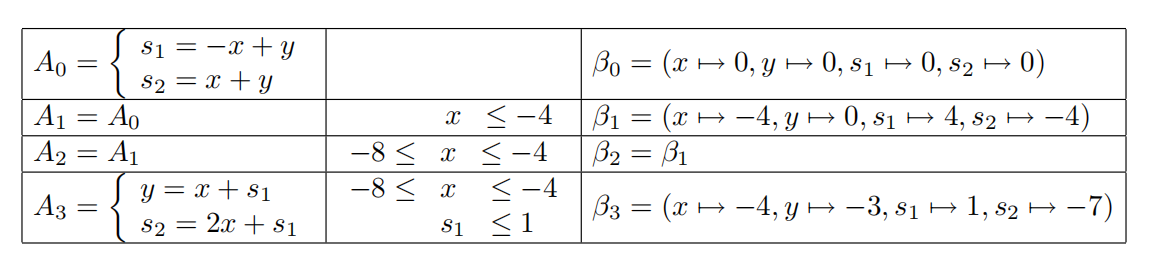
\includegraphics[width=1\linewidth]{4.png}
	\end{figure}
\end{frame}

\section{Strict Inequalities}
\begin{frame}
	\frametitle{Conversion to non-strict Inequalities}
	\begin{lemma}
		A set of linear arithmetic literals $\Gamma$ containing strict inequalities $S=\left\{p_{1}>0, \ldots, p_{n}>\right.$ $0\}$ is satisfiable iff there exists a rational number $\delta>0$ such that for all $\delta^{\prime}$ such that $0<\delta^{\prime} \leq \delta$, $\Gamma_{\delta}=\left(\Gamma \cup S_{\delta}\right) \backslash S$ is satisfiable, where $S_{\delta}=\left\{p_{1} \geq \delta, \ldots, p_{n} \geq \delta\right\}$
	\end{lemma}
	Rather than computing an explicit value for $\delta$, we treat it symbolically, as an \emph{infinitesimal parameter}.
\end{frame}

\begin{frame}
	\frametitle{$\mathbb{Q}_{\delta}$}
	A pair $(c, k)$ of $\mathbb{Q}_{\delta}$ is denoted by $c+k \delta$ and the following operations and comparison are defined in $\mathbb{Q}_{\delta}$:
	$$
	\begin{aligned}
		\left(c_{1}, k_{1}\right)+\left(c_{1}, k_{2}\right) & \equiv\left(c_{1}+c_{2}, k_{1}+k_{2}\right) \\
		a \times(c, k) & \equiv(a \times c, a \times k) \\
		\left(c_{1}, k_{1}\right) \leq\left(c_{2}, k_{2}\right) & \equiv\left(c_{1}<c_{2}\right) \vee\left(c_{1}=c_{2} \wedge k_{1} \leq k_{2}\right)
	\end{aligned}
	$$
\end{frame}

\begin{frame}
	\frametitle{Conversion to non-strict Inequalities}
	And the transformation rules are such as:
	\begin{figure}[htbp]
		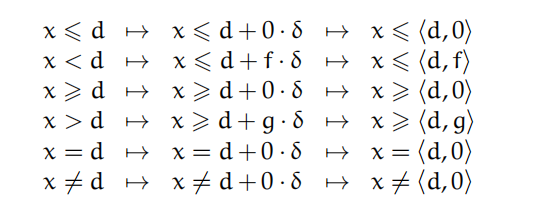
\includegraphics[width=.7\linewidth]{9.png}
	\end{figure}
	where $f<0,g>0$
\end{frame}

% \begin{frame}
% 	\frametitle{Check}
% 	\begin{columns}
% 		\begin{column}{.4\textwidth}
% 			\begin{figure}[htbp]
% 				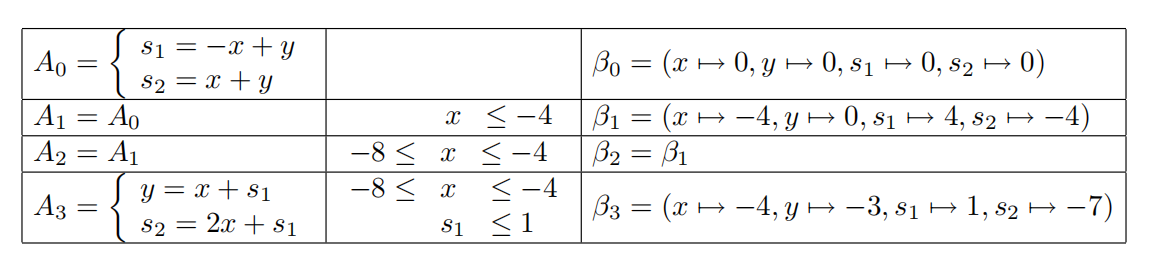
\includegraphics[width=1\linewidth]{4.png}
% 			\end{figure}
% 		\end{column}

% 		\begin{column}{.6\textwidth}
% 			\begin{itemize}
% 				\item If there is a violated linear constraint, perform a simplex step.
% 				\item If there is a violated piecewise-linear constraint, attempt to fix it.
% 				\item If a piecewise-linear constraint had to be fixed more than a certain number of times, perform a case split on that constraint.
% 				\item If the problem has become unsatisfiable, undo a previous case split (or return UNSAT if no such case split exists).

% 				\item  Return SAT (all constraints are satisfied).
% 				\item  Deduction: heuristics
% 			\end{itemize}
% 		\end{column}

% 	\end{columns}
% \end{frame}

\section{Integer and Mixed Integer Problems}
\begin{frame}
	\frametitle{Branch and Bound}
	For constraints:
	\begin{equation}
		\begin{aligned}
			A x &=0 \\
			l_{j} \leq x_{j} & \leq u_{j} \text { for } j=1, \ldots, n
		\end{aligned}
	\end{equation}

	\begin{itemize}
		\item First,solving the linear programming relaxation to get $\beta\left(x_{i}\right)$.
		\item For $c <\beta\left(x_{i}\right) <c+1$ is not integer, the original problem $S$ is split into the following
		two subproblems: 
	\end{itemize}
\end{frame}

\begin{frame}
	\frametitle{Branch and Bound}
	\begin{figure}[htbp]
		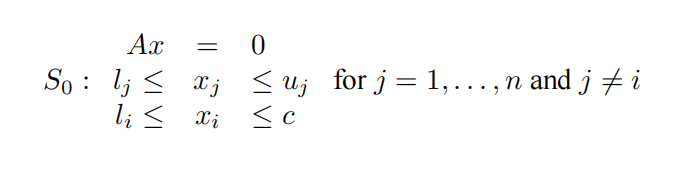
\includegraphics[width=.5\linewidth]{6.png}
	\end{figure}

	\begin{figure}[htbp]
		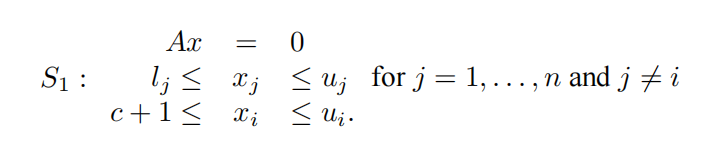
\includegraphics[width=.5\linewidth]{7.png}
	\end{figure}
\end{frame}

\begin{frame}
	\frametitle{Gomory Cuts}
	\begin{itemize}
		\item Assume $\beta$ is a solution to the LP-relaxation $P'$ of $S$ but not a solution
		to $S$. A \emph{cut} is a linear inequality:
		$$
		a_{1} x_{1}+\ldots+a_{n} x_{n} \leq b
		$$

		\item If one or more such cuts can be found, then they can be added as new constraints to the original problem $S$. This
		gives a new problem $S'$ that has the same solutions as $S$ but whose LP-relaxation $P'$ is strictly more
		constrained than $P$.
	\end{itemize}
\end{frame}

\begin{frame}
	\frametitle{Gomory Cuts}
	\begin{figure}[htbp]
		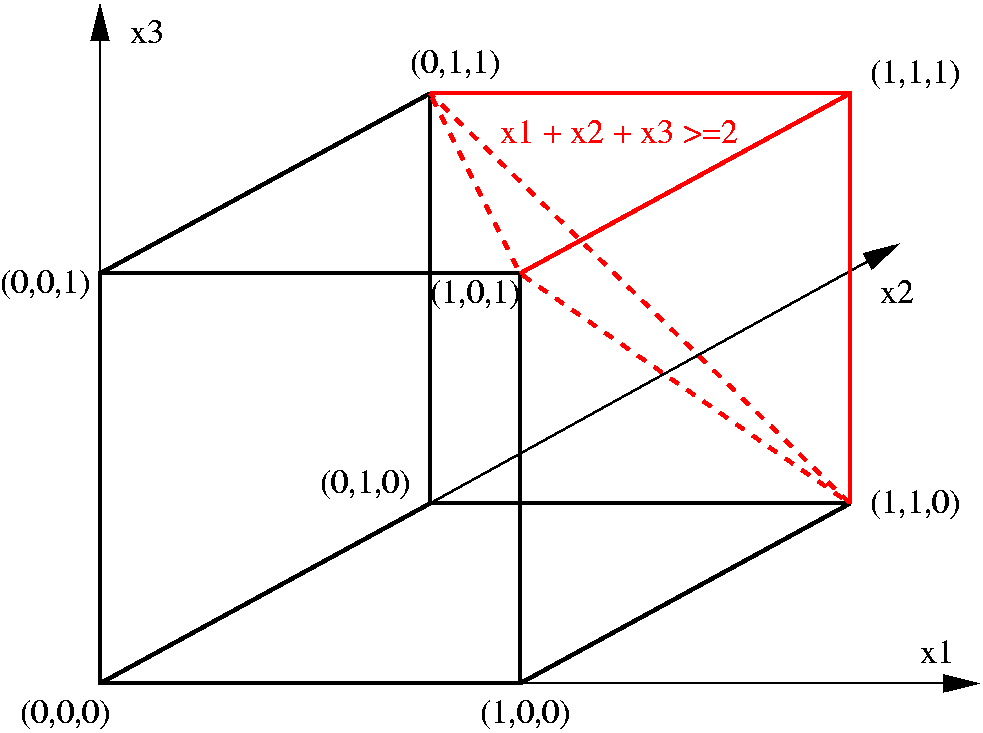
\includegraphics[width=.5\linewidth]{8.png}
	\end{figure}
\end{frame}

\section{Experiments}
\begin{frame}
	\frametitle{Experiments}
	\begin{figure}[htbp]
		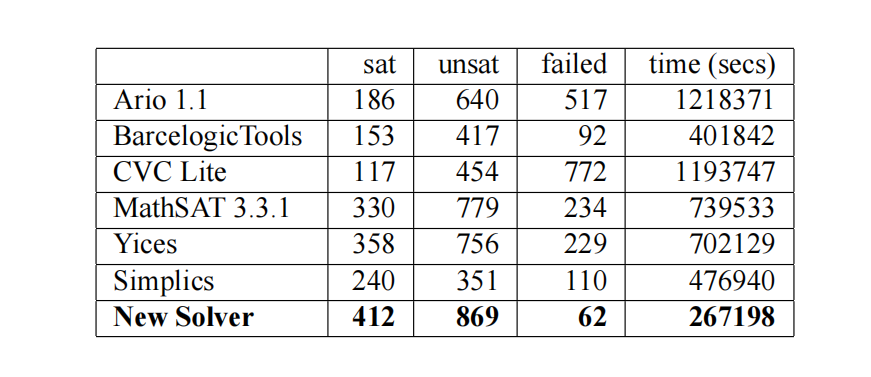
\includegraphics[width=.7\linewidth]{5.png}
	\end{figure}
	\begin{itemize}
		\item  Efficient backtracking and the presimplification
		\item  Efficient theory propagation based on bound refinement
	\end{itemize}
\end{frame}



%------------------------------------------------


%------------------------------------------------

%------------------------------------------------


%------------------------------------------------
\begin{frame}
\hfill
\center{\Huge{\calligra{\Huge{Thank you}}}}
\linespread{3}\selectfont
\end{frame}
%----------------------------------------------------------------------------------------
\end{document}